\documentclass[a4paper]{article}

\newif\ifdraft
\drafttrue
%\draftfalse

\usepackage{graphicx}
\usepackage{twocolpceurws}
\usepackage{xspace}
\usepackage{color}
\usepackage[usenames,dvipsnames]{xcolor}
\usepackage{hyperref}

\ifdraft
  \newcommand{\grex}[1]{{\color{red}\emph{Gregorio says: #1}}\xspace}
    \newcommand{\rnombela}[1]{{\color{blue}\emph{Roberto says: #1}}\xspace}
  \newcommand{\cn}{\textcolor{pink}{[citation needed]}}
\else
  \usepackage[disable]{todonotes}
  \newcommand{\grex}[1]{}
  \newcommand{\rnombela}[1]{}
  \newcommand{\fixme}[1]{}
  \newcommand{\cn}{}
\fi

\let\labelindent\relax
\usepackage[inline]{enumitem}

\newcommand{\RQ}[1]{\emph{RQ\textsubscript{#1}}}
\newcommand{\HP}[1]{\emph{H\textsubscript{#1}}}
%\newlist{rquestion}{enumerate}{2}
%\setlist[rquestion,1]{label=\RQ{\arabic*.}, itemsep=0cm, topsep=0.1cm, leftmargin=3.4em}
%\setlist[rquestion,2]{label*=\emph{\textsubscript{\arabic*.}}, itemsep=0cm, topsep=0cm, leftmargin=2.6em}

\newcommand{\tbd}{\emph{To be done.}}

\newenvironment{hassanbox}%
{\begin{center}\vspace{1mm}\noindent\begin{Sbox}\begin{minipage}{0.95\columnwidth}}%
{\end{minipage}\end{Sbox}\fbox{\TheSbox}\end{center}\vspace{1mm}}

%%% Local Variables:
%%% mode: latex
%%% TeX-master: "fairness"
%%% End:


\title{A Preliminary Quantitative Analysis of App Inventor Projects}

\author{
Roberto Nombela \\ Universidad Rey Juan Carlos\\
                Madrid, Spain \\ r.nombelaa@alumnos.urjc.es
\and
Gregorio Robles \\Universidad Rey Juan Carlos \\
                Fuenlabrada, Madrid, Spain \\grex@gsyc.urjc.es
}

\institution{}

\begin{document}
\maketitle

\begin{abstract}
Visual programming languages help learners to acquire and improve programming and computational skills.
There are many visual programming languages and platforms currently, being Scratch the most popular one.
After Scratch, learners usually move to other visual languages, as for instance MIT App Inventor, a visual programming language block-based to create Android applications.
Many studies exist on the acquisition and assessment of computational thinking skills in Scratch.
However, despite its wide use, similar studies on the use of App Inventor can be seldom found.
That is why in this paper we gather and analyze App Inventor projects with the goal of having an overview of the type of projects that are created.
Our aim in the long run is to create tools that support the learning process of App Inventor.
\end{abstract}


\section{Introduction}
In recent years, the concept of Computational Thinking (CT) has been presented as a process to solve problems, not necessarily only in programming~\cite{wing2006computational}. 
CT includes skills that facilitate the resolution of problems, such as: abstraction, algorithmic and parallel thinking, data representation. These abilities make the CT a fundamental help for any learner.

One way to acquire and improve the skills of CT and programming level are visual programming languages.
This is because programming involves activities such as the ability to design, create and invent new media~\cite{resnick2009scratch}.
The Scratch and App Inventor visual programming languages are examples of this.

Because of this, tools that assess the CT skills from the projects of these programming languages have also emerge, for example Dr. Scratch~\cite{moreno2015dr} and Code Master that analyze the Scratch and App Inventor (and Snap!) projects respectively. 
At current time, these assessments have turned out to be more useful for educators than for learners by the fact that the latter do not receive enough feedback to improve~\cite{robles2018ontools}.

This study aims to find a way to help learners improve by analyzing the blocks of App Inventor projects. Observing values as number or variety of blocks we will have an overview of the type of projects that the App Inventor community are creating.

For the analysis, more than 1000 projects obtained from the Gallery of App Inventor web have been used. 
In this Gallery you can find tens of thousands of projects uploaded by users. The age, gender, nationality or level of programming of the users are unknown.

This paper is structured as follows: the first section is an introduction to MIT App Inventor. Then, the Methodology section talks about the acquisition and preparation of the data for the analysis and the Results section shows and explains what has been obtained using the cleaned data. Finally, the Future work section mentions possible improvements to the CT assistance tools.

\section{MIT App Inventor}
MIT App Inventor is a visual programming language block-based to create Android applications. Users can build their apps by dragging and dropping the components. There are two modes, \emph{Designer} and \emph{Blocks}. In Designer mode, the User Interface is created with elements such as Buttons, Images, Canvas... In Blocks mode, users specify the behavior of the app by joining blocks like completing a puzzle~\cite{wolber2011app}.

In the App Inventor documentation web page\footnote{\url{http://appinventor.mit.edu/explore/ai2/support/blocks.html}} there are 8 families of blocks: control, logic, math, text, list, color, variable and procedures. Table~\ref{tab:block-fam} shows the different families and what each one can include. In addition to these 8 families there is one more: Components. This family is composed of all the elements that can be used in App Inventor to create applications. Each component can have methods, events and properties.

\begin{table}
\begin{center}
\caption{Blocks families and properties}
\bigskip
\label{tab:block-fam}
\begin{tabular}{|l|l|}
\hline
\textbf{Control} & Conditionals, loops... \\ \hline
\textbf{Logic} & True, false, and, or... \\ \hline
\textbf{Math} & Numbers, operations\\ \hline
\textbf{Text} & String functions\\ \hline
\textbf{List} & List functions\\ \hline
\textbf{Color} & Color box, make or split color \\ \hline
\textbf{Variable} & Initialize/Set/Get variable\\ \hline
\textbf{Procedure} & Do/Result\\ \hline
\end{tabular}
\end{center}
\end{table}

\begin{figure}
\begin{center}
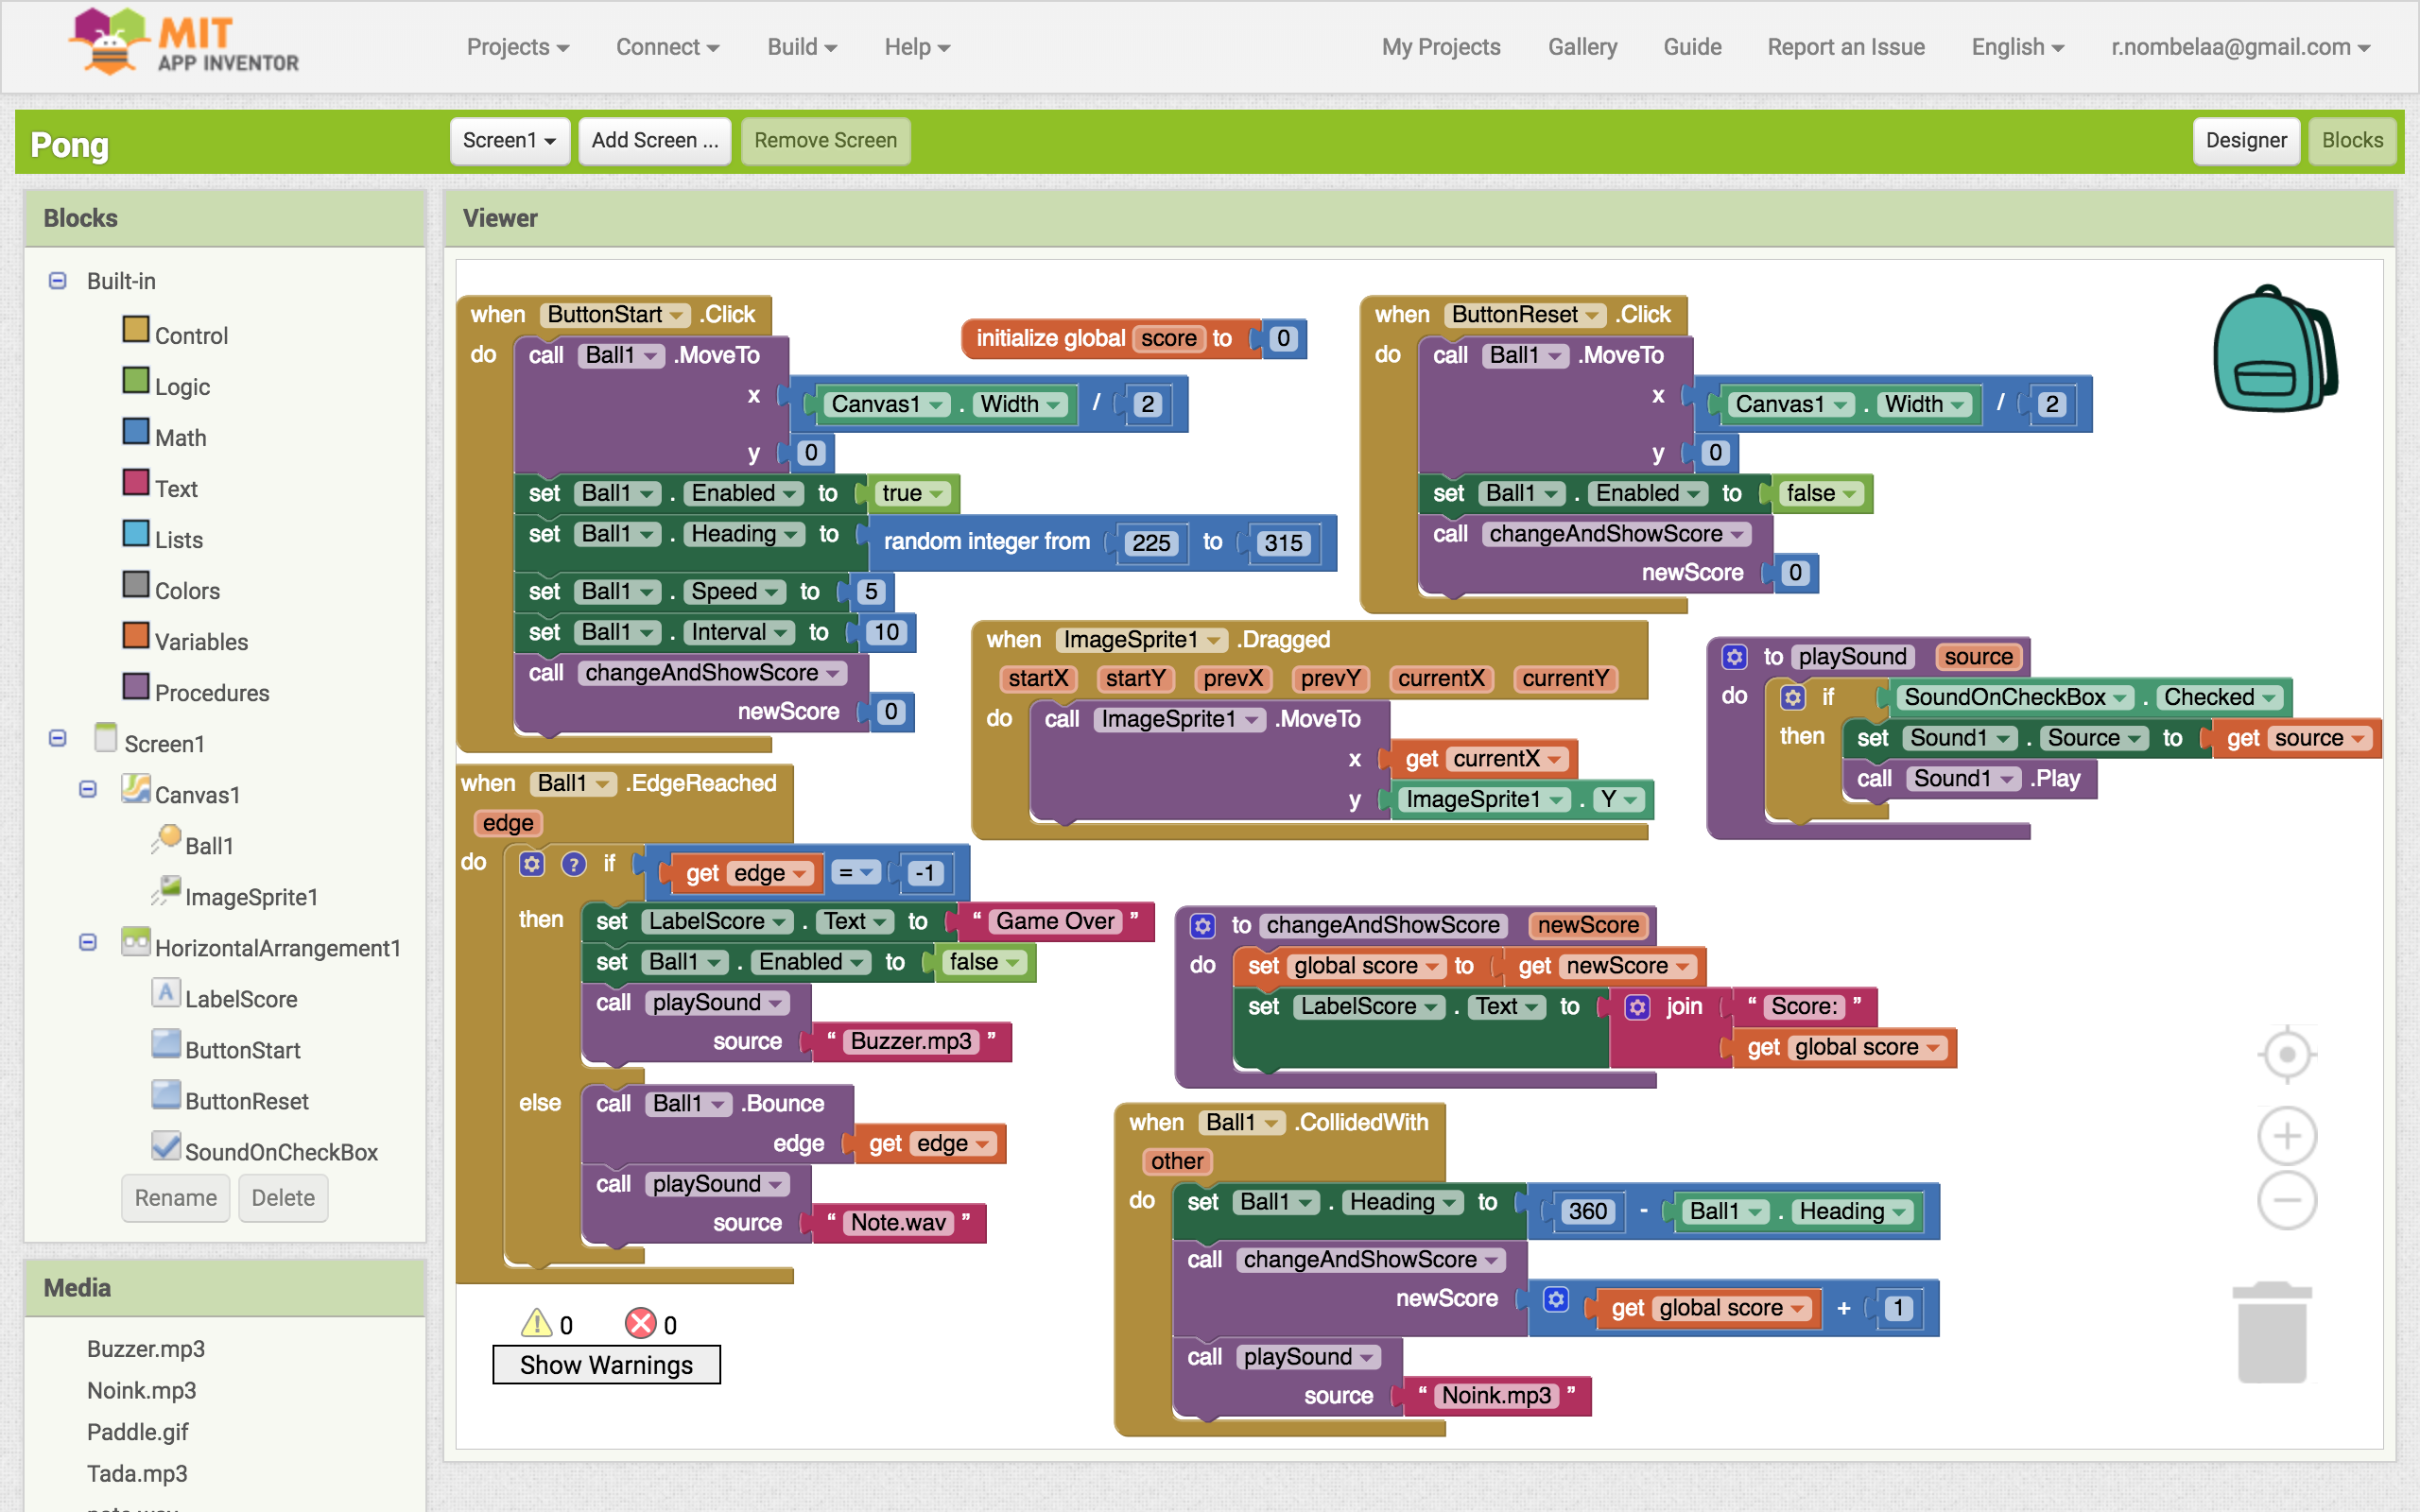
\includegraphics[height=5cm]{blocks-example}
\caption{Blocks mode screenshot.}
\label{fig:blocks-example}
\end{center}
\end{figure}

In Figure~\ref{fig:blocks-example}, we have the App Inventor Blocks mode screen for a Pong game application. Each family of blocks is identified with a different color. This app uses all the classes, except Colors and Lists. Control blocks handle events, like when a button is clicked. Logic blocks, true and false, enable or disable the ball. Math blocks set the position of the ball. Text blocks set the text ``Game Over" in a label. Variables blocks set the score. Procedures blocks are called to make sounds or move the ball.

\begin{figure}
\begin{center}
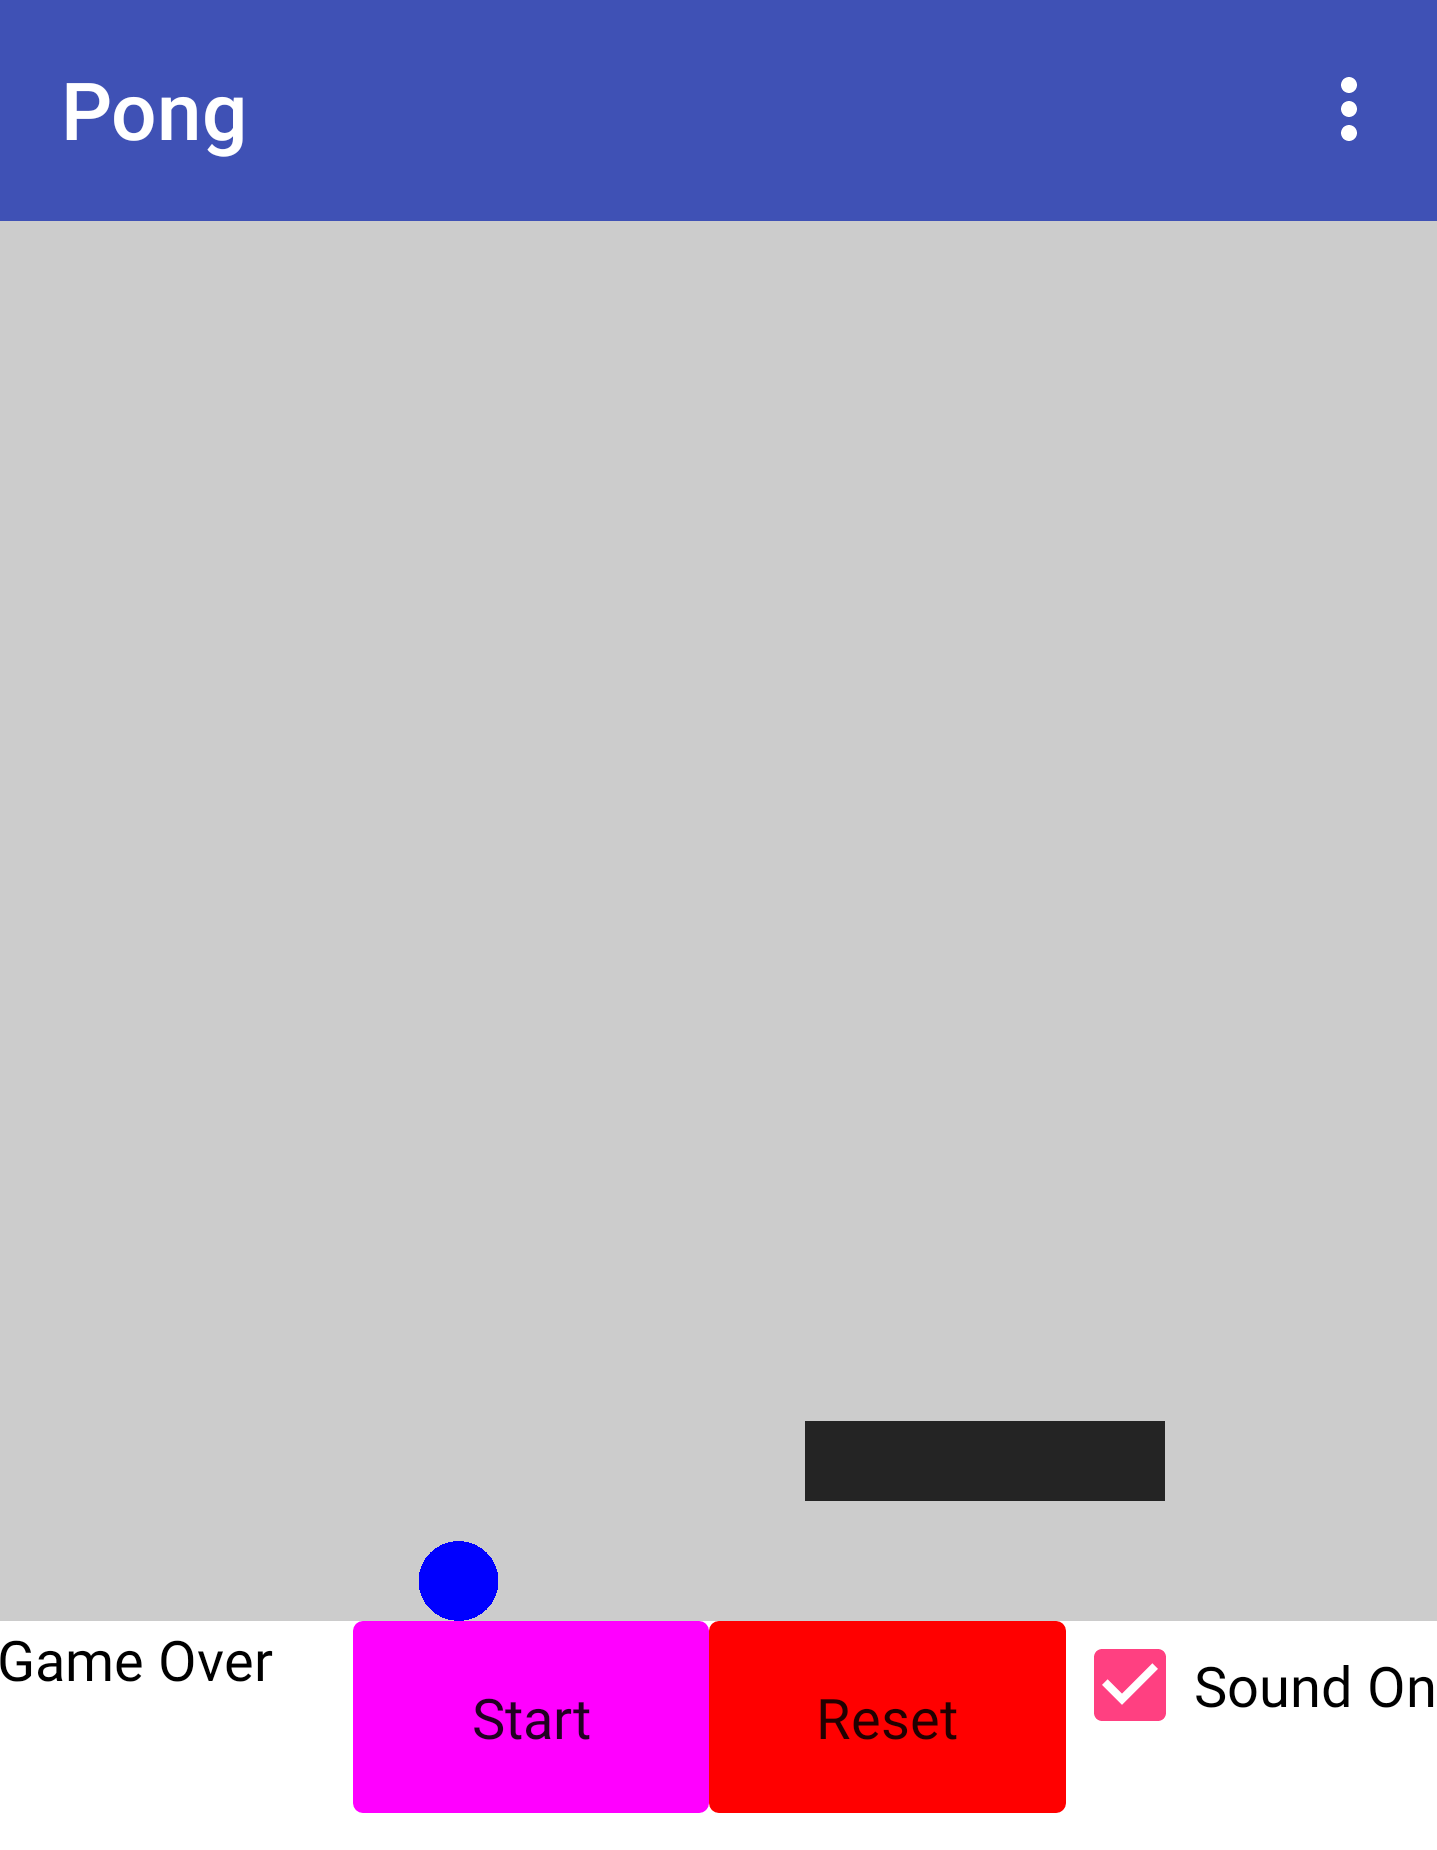
\includegraphics[height=5cm]{app-screen}
\caption{App screenshot of a Pong game.}
\label{fig:app-example}
\end{center}
\end{figure}

Figure~\ref{fig:app-example} shows a screenshot of the Pong game in the built-in app. Some of the previously mentioned components can be seen: the ball, one image as the paddle, the ``Game Over" label because the ball is on the floor, two buttons to start and to reset and one check box.

\section{Methodology}
\subsection{Data Gathering}
The process of data gathering consists of downloading projects from the App Inventor Gallery. In addition to the most popular projects, the most recent ones have also been downloaded, since many projects are being uploaded every day. One problem with this is that you can find many empty (0 blocks) or duplicate projects. Another problem is the difficulty to automate the download process because you have to make a copy of the Gallery projects to your account projects and then download them. All compressed projects can be found on GitHub\footnote{\url{https://github.com/robernom/app-inventor-analysis/blob/master/AI_projects.zip}}.

Every project has two different types of files per screen, \emph{bky} and \emph{scm}. The bky files contain, in XML format, all the blocks used. On the other hand, scm files use a JSON structure and represent all the components used. Thus, to extract the blocks we run a script that creates a dictionary where the key is the type and the value is the number of blocks of that type, looks at the next block and if it is a new type it is included to the dictionary with value one, otherwise it is added one to the value. Using this script for each project we have all the blocks extracted and classified, so this information is saved in a CSV file. Once we have all projects prepared, we must discard empty or duplicate projects. 

Table~\ref{tab:blocks} shows how the discarding of invalid projects affects the number of blocks. Initially, we had 1222 projects that became 1102 when we remove empty projects and, in the end, we had 730 projects by eliminating duplicate projects. While, unlike the number of projects, the mean, the median and the standard deviation increase their values. Logically, when empty projects are removed, the minimum becomes 1.

\subsection{Data analyzing}
In order to assess the CT of the projects, we use our own tool called Dr. App Inventor. This tool is an analogy of Dr. Scratch to analyze App Inventor projects while using the Code Master rubric\footnote{\url{http://apps.computacaonaescola.ufsc.br:8080/rubrica_appinventor.jsp}}, written in Python.

The algorithm of the tool receives the file with the project and decompresses it. Inside the file there are 3 directories: \emph{assets} contains the media files; \emph{youngandroidproject} has the project properties like the project name or the app name; and \emph{src}, which includes the bky and scm files, mentioned previously.

In the bky, the tool extracts the blocks and then classifies them according to the type, while in the scm it collects all the components. Once Dr. App Inventor has identified the blocks and components, it applies the rubric and returns the score for each criterion along with the total score.

\begin{table}
\begin{center}
\caption{Comparative table of the number of blocks}
\bigskip
\label{tab:blocks}
\begin{tabular}{|l|r|r|r|}
\hline
& Original & Non-empty & No duplicate \\ \hline
Projects & 1,222 & 1,102 & 730\\ \hline
Mean & 187.89 & 208.35 & 211.48\\ \hline
Std. Dev & 463.68 & 483.9 & 502.62 \\ \hline
Median & 47 & 55 & 60\\ \hline
Minimum & 0 & 1 & 1\\ \hline
Maximum & 5,476 & 5,476 & 5,476 \\ \hline
\end{tabular}
\end{center}
\end{table}

Next, the ``used blocks'' are studied, that is, each type of block adds one for each project in which it has been used. The ``repeated blocks'' are also studied: we add the number of each type of blocks used in each project. We can see that the correlation of both is 0.84, which means that they are highly related.

\section{Results}
\subsection{Study of the blocks usage}
Table~\ref{tab:block-fam-comp} gives a count of all the blocks according to their family to sort families according to their usage. Component is the most used while Color is the least, this is logical because an application needs more a button or a media player, for example, than any color.

\begin{table}
\begin{center}
\caption{Comparison of the use of the families}
\bigskip
\label{tab:block-fam-comp}
\begin{tabular}{|l|r|}
\hline
\textbf{Family} & \textbf{Frequency} \\ \hline
Component & 49,507 \\ \hline
Text	& 25,426\\ \hline
Math & 24,862\\ \hline
Variables & 21,765\\ \hline
Logic & 12,792\\ \hline
Control & 8,915\\ \hline
Lists & 4,381\\ \hline
Procedure & 4,282\\ \hline
Colors & 2,452\\ \hline
Total & 154,382\\ \hline
\end{tabular}
\end{center}
\end{table}

\begin{table}[ht]
\begin{center}
\caption{Number of blocks statistics}
\bigskip
\label{tab:number-blocks}
\begin{tabular}{|l|r|}
\hline
Types & 107\\ \hline
Mean & 1,442.82\\ \hline
Std. Dev & 4,232.51\\ \hline
Median & 133\\ \hline
Minimum & 1\\ \hline
Maximum & 28,927\\ \hline
Total & 154,382\\ \hline
\end{tabular}
\end{center}
\end{table}

Looking at all the blocks now, Table~\ref{tab:number-blocks} shows the statistics of the times that the blocks are used in the 730 valid projects. The mean is 1,442.82 and there is a big standard deviation. The median is 133, that is, of the 107 types of blocks at least 50\% of them are used 133 times.

Table~\ref{tab:most-least} shows the most used blocks independently of their family.

\begin{table}
\begin{center}
\caption{Most and less used blocks}
\bigskip
\label{tab:most-least}
\begin{tabular}{|l|r|}
\hline
component\_set\_get & 28,927\\ \hline
text & 22,644\\ \hline
math\_number & 15,308\\ \hline
lexical\_variable\_get & 14,662\\ \hline
component\_event & 9,599\\ \hline
... & ... \\ \hline
list\_to\_csv\_table & 3\\ \hline
math\_tan & 2\\ \hline
obfuscated\_text & 2\\ \hline
text\_is\_string & 2\\ \hline
controls\_closeScreenWithPlainText & 1\\ \hline
\end{tabular}
\end{center}
\end{table}

The most used block is \emph{component\_set\_get}, whose function is to introduce or obtain the properties of a component. The following is \emph{text}, which is used to create strings. \emph{Math\_number} can take the value of any positive or negative number (decimals included). \emph{Lexical\_variable\_get} provides the value of any variable. \emph{Component\_event} takes the value of any event that belongs to the component.
These blocks represent a large percentage of their families. Components: 77.82\%; Text: 89.06\%; Math: 61.57\%; Variable: 67.37\%.

Between the least used blocks we can find \emph{list\_to\_csv\_table} which converts a list in a CSV, \emph{math\_tan} returns the tangent of the given number in degrees, \emph{obfuscated\_text} provides security if there is confidential information in the app, \emph{text\_is\_string} returns true if the parameter is a string and \emph{controls\_closeScreenWithPlainText} closes the current screen and passes text to the app that opened this one. These blocks are less used because they are very specific for the common applications.

In order to know which are the most and least used blocks in low diversity projects, in Table~\ref{tab:most-least-low} we calculate them for projects with a variety less than 10.

\begin{table}[ht]
\begin{center}
\caption{Most and less used blocks for low diversity projects}
\bigskip
\label{tab:most-least-low}
\begin{tabular}{|l|r|}
\hline
component\_set\_get & 5,562\\ \hline
text & 4,538\\ \hline
component\_event & 3,960\\ \hline
component\_method & 3,484\\ \hline
controls\_openAnotherScreen & 1,277\\ \hline
... & ... \\ \hline
text\_trim & 0\\ \hline
math\_divide & 0\\ \hline
math\_cos & 0\\ \hline
controls\_forEach & 0\\ \hline
math\_convert\_number & 0\\ \hline
\end{tabular}
\end{center}
\end{table}

The two first blocks are the same that we obtained for all the projects. \emph{Component\_event} is the third while before it was the fifth. Now, we have \emph{component\_method} that refers to any method that can be used by the component and \emph{controls\_openAnotherScreen} which opens the screen with the provided name.

By knowing which are the most and least used blocks or families of blocks, educators will be able to give more emphasis to ones than others. Furthermore, if there are some that are underutilized, they can explain these with more attention.

For example, Control and Procedure families are essential tools for CT since they participate in algorithmic thinking and procedural abstraction but they only represent 5.77\% and 2.77\% of the total, respectively. This may be a potential learning gap and students should consider these types of blocks further.

\subsection{Study of the scores depending on the variety}

The variety of a project is the number of different types of blocks used. This study aims to confirm what intuition suggests: the more variety a project has, the higher the score. 
Figure~\ref{fig:var-dist} presents the distribution of the variety. The x axis represents the variety of each project and the y axis represents the frequency or the times a variety is given. The figure reveals that most projects have a relatively low variety. We can see that the predominant values are between 3 and 6, in addition there are some projects around 50 and an isolated project with 61 different blocks. 

\begin{figure}
\begin{center}
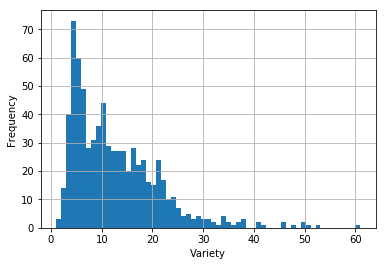
\includegraphics[height=5cm]{fig1}
\caption{Distribution of the variety}
\label{fig:var-dist}
\end{center}
\end{figure}

Projects with more than 10 different blocks represent 48.2\% (352 of 730) of the blocks and the scores can be characterized as seen in Table~\ref{tab:comparison} versus the scores of the projects with less than 10 different blocks. Projects with high diversity almost double in all respects to those with low diversity. This means that the initial hypothesis is true.

\begin{table}
\begin{center}
\caption{Scores in low and high diversity projects}
\bigskip
\label{tab:comparison}
\begin{tabular}{|l|r|r|}
\hline
& High diversity & Low diversity \\ \hline
Projects & 352 & 378\\ \hline
Percentage & 48.2 & 51.8\\ \hline
Mean & 18.56 & 9.89\\ \hline
Std. Deviation & 5.33 & 3.27\\ \hline
Median & 18 & 10\\ \hline
Minimum & 7 & 3\\ \hline
Maximum & 36 & 19\\ \hline
\end{tabular}
\end{center}
\end{table}

The results of the projects according to the variety allow us to get an idea of the need to use different blocks before a large number of blocks. For example, Table~\ref{tab:comp-num-var} shows the comparison of the project with the largest number of blocks versus the most varied. Once again, we can see the straight relationship between variety and score.

\begin{table}
\begin{center}
\caption{Comparison of quantity versus variety}
\bigskip
\label{tab:comp-num-var}
\begin{tabular}{|r|r|r|}
\hline
Number & Variety & Score \\ \hline
5476 & 16 & 18\\ \hline
4115 & 61 & 36\\ \hline
\end{tabular}
\end{center}
\end{table}

\section{Future work}
Following the possible enhancements proposed in~\cite{robles2018ontools}, the next step is to get projects for learners to see examples and practice with them. These projects should include Control or Procedure blocks, a high variety or the combination of both. 

Another step is to provide personalized feedback based on each student's progress and needs. For this purpose, the projects of the learner could be analysed in a similar way to the analysis carried out in this study.

\section*{Acknowledgements}
This research has been supported in part 
by the Region of Madrid under project ``eMadrid:
Investigaci\'on y Desarrollo de tecnolog\'ias educativas en la
Comunidad de Madrid'' (S2013/ICE-2715).


\bibliographystyle{plain} 
\bibliography{samplebib}
%inline the .bbl file directly for mailing to authors.

\end{document}


